Das nächste Grundlagenkapitel listet Erfolgschancen für Unternehmen auf, die Cloud-Dienste in ihre Geschäftsprozesse integrieren.

\begin{flushleft}
      Es wird erklärt warum die Kostenoptimierung und -überwachung relevant für Unternehmen sind.
\end{flushleft}


Die Optimierungsergebnisse können zu folgenden Ergebnissen führen.
\begin{itemize}
      \item
            Die Möglichkeit, die individuellen Kosten verschiedener Projekte die über dieselbe Infrastruktur laufen, zu erkennen. Auf diese Weise ist es auch möglich, zwischen Kunden, die mehr Ressourcen verbrauchen, und solchen, die weniger verbrauchen, zu unterscheiden.
      \item
            Eine beachtliche Erhöhung der (finanziellen) Rentabilität im Unternehmen.
      \item
            Eine geringere Unsicherheit, bei der Umsetzung von cloudbasierten Systemen.
      \item
            ...
\end{itemize}

%Basandose en "Vor- und Nachteile der Nutzung von Cloud-Diensten (mit mobilen Endgeräten) in Organisationen und deren Einfluss auf die Nachhaltigkeit"
% Debería aclarar los aspectos principales de mi BA
% En mi caso: 

%1-Cuales son los miedos, razones y oportunidades para las empresas en la NUBE?

%\subsection{Risiken und Oportunitäten der Cloud...}\label{subsec_UabsGrund2}
%Vor- und Nachteile / ?

\subsection{Ökonomie des Cloud Computing}\label{subsec_UabsGrund3}
%Was bietet die Cloud den Unternehmen?
%Economics of Cloud Computing
%https://d1.awsstatic.com/whitepapers/introduction-to-aws-cloud-economics-final.pdf
[to check:]
\begin{flushleft}
      {
            Cloud Economics auf Englisch, basiert auf das On-Demand Prinzip basiert,
            gibt die Flexibilität, Rechnerkapazität je nach Bedarf entweder manuell oder automatisch anzupassen.
            Es entfallen große Investitionen in Hardware, wie bei On-Premise-Systemen.
            Durch den Verzicht auf Hardware entfallen die Kosten für Reparatur, Wartung und eventuell damit verbundene Lizenzen, und im Falle von Systemen, die dies benötigen, entfällt der Bedarf an zuständigem Personal.

            Die Nutzung dieser Dienste ist innerhalb weniger Minuten und selbstständig möglich (Selbsbedienung). }
\end{flushleft}

Grafik der Kosten On-Premise/Demand?

\subsection{Skalierbarkeit}
Mit Auto Scaling ist es möglich sicherzustellen, dass die Anzahl der Amazon Server-Instanzen während
Nachfragespitzen nahtlos hochskaliert werden, um die Leistung aufrechtzuerhalten, und in
Nachfrageflauten automatisch reduziert wird, um die Kosten zu minimieren.
Auf diese Weise kann es weniger Zeit mit der Verwaltung von IT-Ressourcen verbracht werden und sich mehr auf ihr Geschäft konzentrieren können.
\\\\
Das war der Fall von Walgreens in der USA.
Sie haben unter anderen 750 virtuelle Maschinen und SAP HANA auf Azure Instanzen migriert.

\begin{quote}
      „One of the key reasons for moving to Azure was so that we could take advantage of the scalability that SAP HANA is capable of„
      \\
      Dan Regalado: Vice President of Global Technology Transformation and Strategic Partnerships Walgreens Boots Alliance
            {\cite{AZ01}}
\end{quote}

\subsection{Flexibilität und Agilität}

\subsection{Selbstbedienung}

\subsection{Keine Vorabkosten}
%https://aws.amazon.com/de/ec2/pricing/
Amazon Web Services bietet ein Pay-as-you-go-Modell für Ressourcen in On-Demand Zahlungsmodel.
Diese werden nach einen bestimmter Einheit wie GB/Stunde berechnet für Speichereinheiten. 
\\
Im Fall von Server-Instanzen wird es ein Stundensatz auf der Grundlage der Servereigenschaften festgelegt.  

Hier einige Beispiele von EC2-Instanzen l.

\begin{center}
      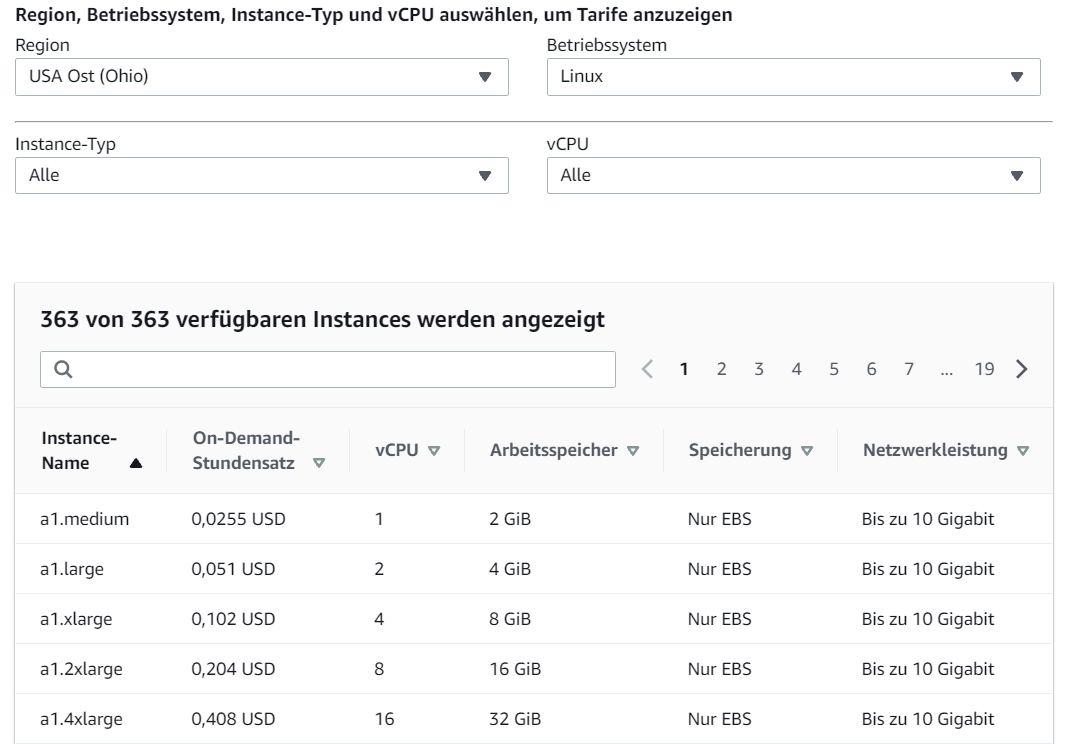
\includegraphics[scale=0.4]{sources/On-Demand-Pläne für Amazon EC2}\label{fig:OnDemand_Preise}\\
      \textbf{Abbildung \autoref{fig:OnDemand_Preise}:} On-Demand Preise für Amazon EC2
      \footnote{Vgl. u.a.\cite{AMZ01}}
  \end{center}

\begin{comment}
Advantages of Cloud Technology
As the technology has matured over the last decade, companies are moving to the
cloud to lower costs, reduce complexity, and increase flexibility. The cloud
provides scalable and powerful compute solutions, low-cost, reliable storage, and

addition, cloud technologies can be used to deploy solutions quickly and cost effectively around the world and on any device.
When you decouple from the data center, you’ll be able to:
x Decrease your TCO: Eliminate many of the costs related to building and
maintaining a data center or colocation deployment. Pay for only the
resources you consume.

x Reduce complexity: Reduce the need to manage infrastructure,
investigate licensing issues, or divert resources.
x Adjust capacity on the fly: Add or reduce resources, depending on
seasonal business needs, using infrastructure that is secure, reliable, and
broadly accessible.
x Reduce time to market: Design and develop new IT projects faster.
x Deploy quickly, even worldwide: Deploy applications across multiple
geographic areas.
x Increase efficiencies: Use automation to reduce or eliminate IT
management activities that waste time and resources.
x Innovate more: Spin up a new server and try out an idea. Each project
moves through the funnel more quickly because the cloud makes it faster
(and cheaper) to deploy, test, and launch new products and services.
x Spend your resources strategically: Switch to a DevOps model to free
your IT staff from operations and maintenance that can be handled by the
cloud services provider.
x Enhance security: Spend less time conducting security reviews on
infrastructure. Mature cloud providers have teams of people who focus on
security, offering best practices to ensure you’re compliant, no matter what
your industry.
\end{comment}

%\subsection{Was ist EC2? To Review}\label{subsec_UabsGrund4}
%Man kann HW und SW auswählen


% Amazon video Cloud Eco.: https://www.youtube.com/watch?v=kUNBx1MTwxw
% short explaniation https://www.youtube.com/watch?v=RI9RTbXEjLc
%3- Hard and Soft Savings https://youtu.be/Q5wSvUVPyYY?t=316
% Suche ein Buch, mit info darüber!

%\subsection{Dienste für ein Standard-Anwendungsarchitektur}\label{subsec_UabsGrund3}

%4- Etliche Dienste, die gut überwacht werden können und (auch) mit Optimierungsoporunititäten 
\newpage